\section{Pulse Propagation in EIT Media}
  \label{sec:polaritons_propagation}

    In the previous section we considered \textsc{eit} in the $\Lambda$ system
    from the perspective of the medium along with linear response to stationary
    fields. We will now look at the phenomena of \textsc{eit} as it applies to
    the field incident on the medium, in particular the case of pulsed field
    envelopes, using the propagation model developed in chapter
    \ref{chp:propagation}.

    In figure \ref{fig:eit_no_coupling} we show the simulated propagation of a
    Gaussian probe pulse incident on a $\Lambda$-type medium \textit{with the
    coupling field turned off}, \ie $\Omega_c(z=0, \tau) = 0$. In this case the
    pulse has an area $\theta_p = $ \unit[0.2]{$\pi$} and a \textsc{fwhm}
    $\tau_w = $ \unit[1]{$\tau_\Gamma$} (see equation (\ref{eqn:gaussian}) for
    the Gaussian envelope profile). The medium has constant density such that
    the absorption parameters are given by  $N(z) g_{01} = N(z) g_{02} =
    \unit[2\pi~10]{\Gamma/L}$. We see that the pulse is absorbed by the atoms,
    with 50\% of its initial peak amplitude attenuated after travelling a
    distance $\unit[\sim0.2]{L}$ into the medium.

    In figure \ref{fig:eit_coupling} we show the same $\Lambda$-type system but
    this time apply a strong \textsc{cw} coupling field such that $\Omega_c(z =
    0, t) = $ \unit[$2\pi~2$]{$\Gamma$}. This time we see that the pulse suffers
    much less attenuation, with over 50\% of its initial peak amplitude
    transmitted. The introduction of the strong coupling field leads to an
    \textsc{eit} window which allows this transmission of the probe pulse
    through the medium which it would ordinarily find to be opaque.\cite{Fleischhauer2005}

    \begin{figure}[p]
      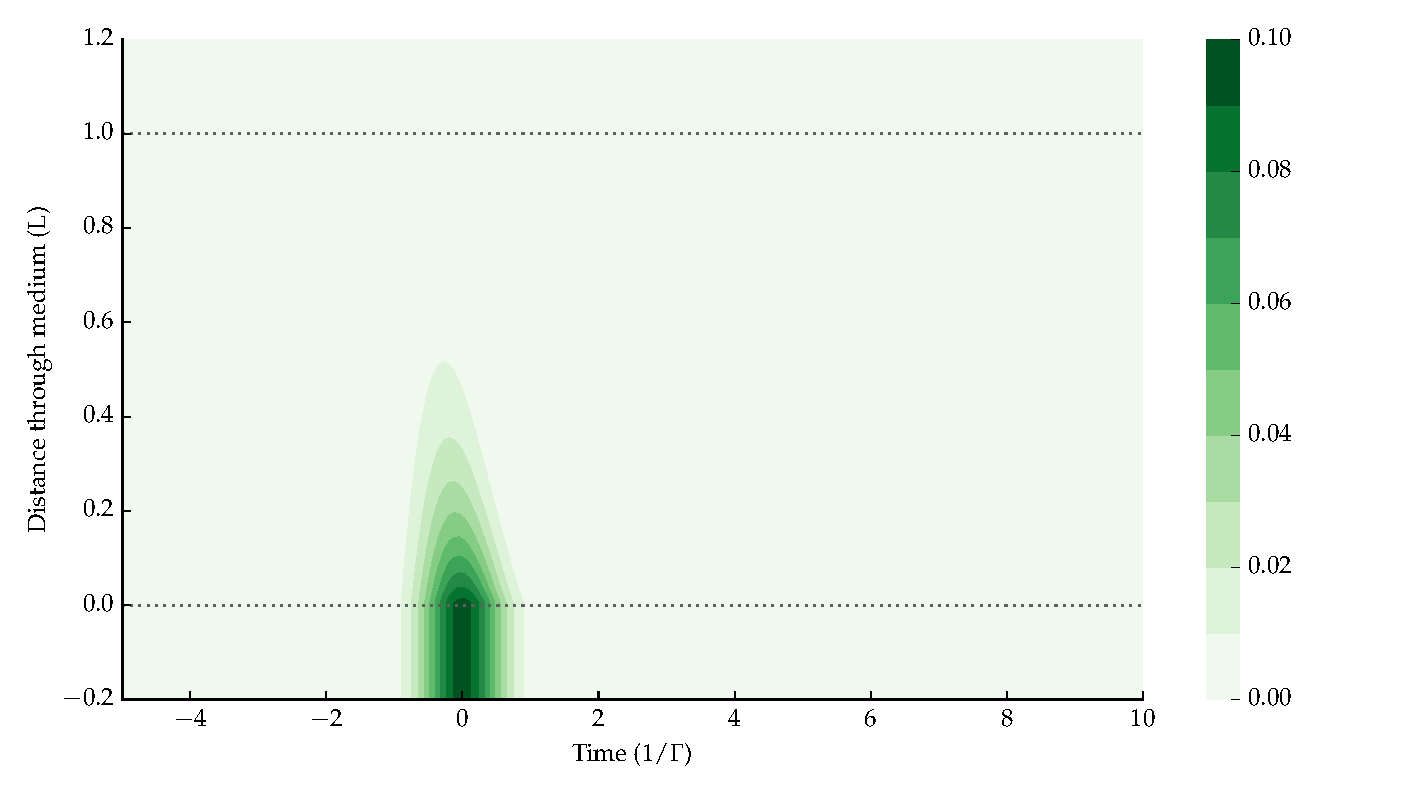
\includegraphics[width=\linewidth]
        {figs/04_polaritons/pls_p0_2pi_t1_Ng1e1_c0_fig1.pdf}
      \caption{
      Simulated absolute value of the complex Rabi frequency $\Omega_p(z, \tau)$
      for the propagation of a Gaussian pulse with area $\theta_p = $
      \unit[0.2]{$\pi$} and \textsc{fwhm} $\tau_w = $ \unit[1]{$\tau_\Gamma$}
      through a $\Lambda$-type medium with constant density such that $Ng =
      \unit[2\pi~10]{\Gamma/L}$. The coupling field is turned off such that
      $\Omega_c(z, \tau) = 0$. The dotted lines at $z = \unit[0, 1]{L}$ mark the
      start and end of the medium.
      }
      \label{fig:eit_no_coupling}
    \end{figure}

    \begin{figure}[p]
      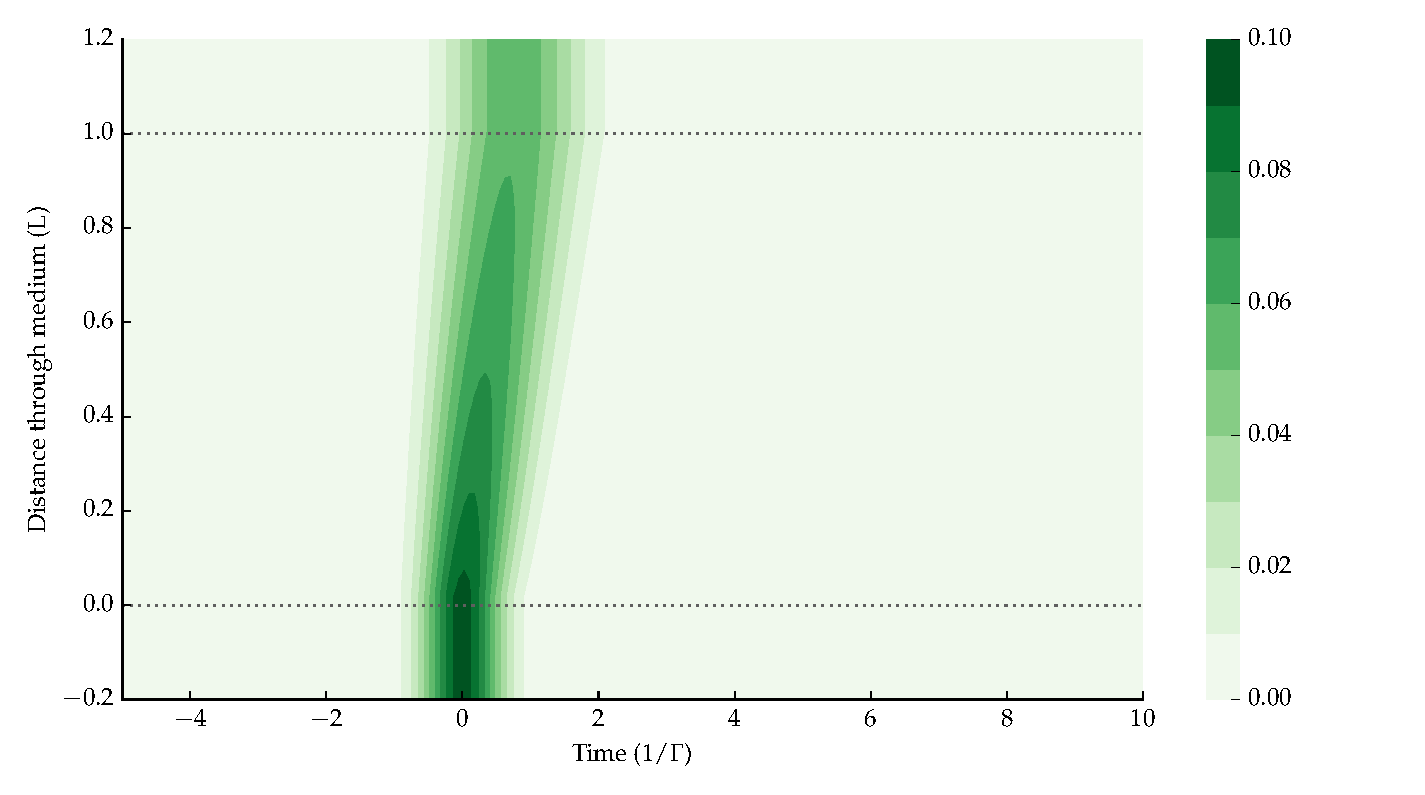
\includegraphics[width=\linewidth]
        {figs/04_polaritons/pls_p0_2pi_t1_Ng1e1_c02_fig1.pdf}
      \caption{
      Simulated absolute value of the complex Rabi frequency $\Omega_p(z, \tau)$
      for the propagation of the same pulse through the same $\Lambda$-type
      medium as figure \ref{fig:eit_no_coupling} but now with a strong
      \textsc{cw} coupling field $\Omega_c = $ \unit[$2\pi~2$]{$\Gamma$}.
      }
      \label{fig:eit_coupling}
    \end{figure}


  \subsection{Group Velocity \& Slow Light}

    In figure \ref{fig:eit_no_coupling} we note that the peak of the pulse moves
    to the left such that it arrives at each position \textit{before} a pulse
    travelling at the vacuum speed of light $c$ would arrive. This is known as
    fast light. Recall that in this speed-of-light reference frame, propagation
    at $c$ is represented by a vertical line.

    [explain why it is OK! No information travels faster than light]

    The group velocity $v_g$ of light travelling in the medium is given by\cite{Fleischhauer2005}
    \begin{equation}
        v_g = \frac{c}{n + \omega_p (\frac{\dd n}{\dd \omega_p})}
        \label{eqn:group_vel}
    \end{equation}

    where $n = \sqrt{1 + \chi_R}$ is the refractive index
    introduced in equation (\ref{eqn:phase_vel_refr}). For the two-level system,
    the familiar frequency-dependent lineshape of the real part of the
    susceptibility $\chi_R$ shown in figure
    \ref{fig:susc_imag_real_linear_comp} demonstrates an anomolous dispersion
    gradient $\dd \chi_R / \dd \omega < 0$ around resonance.

    In contast, in figure \ref{fig:autler_townes} we see that under \textsc{eit}
    conditions, $\dd \chi_R / \dd \omega > 0$ in the transparency window around
    resonance. Equation (\ref{eqn:group_vel}) then tells us that \textsc{eit}
    transmission will be accompanied by a reduction of the group velocity, which
    we indeed observe in figure \ref{fig:eit_coupling}.

    Experiments using \textsc{eit} in Bose-Einstein condensates (\textsc{bec}s)
    have been used to reduce the the speed of light pulses by seven orders of
    magnitude, down to \unit[17]{m s$^{-1}$}.\cite{Hau1999}

  \subsection{Pulse Compression}

    \begin{figure}[h]
      \includegraphics[width=\linewidth]
        % {figs/04_polaritons/pls_p0_2pi_t1_Ng5e3_c10_gaussian_w0_5_2_fig1.pdf}
        {figs/04_polaritons/pls_p0_2pi_t1_Ng5e3_c10_gaussian_w0_5_3_fig2.pdf}
      \caption{
      (Main) Simulated absolute value of $\Omega_p(z, \tau)$ for the propagation
      of a Gaussian pulse with area $\theta_p = $ \unit[0.2]{$\pi$} and
      \textsc{fwhm} $\tau_w = $ \unit[1]{$\tau_\Gamma$} through a $\Lambda$-type
      medium. The medium is of non-uniform density, having a Gaussian profile of
      \textsc{fwhm} \unit[0.5]{L} and a peak density such that $N_{\mathrm{max}}
      g = \unit[2\pi~500]{\Gamma/L}$. The coupling field is \textsc{cw} with
      $\Omega_c = $ \unit[$2\pi~10$]{$\Gamma$}. (Left) Spatial profiles of the
      pulse at different times during the simulation corresponding to vertical
      dotted lines in the main figure. (Inset) Pulse \textsc{fwhm}s
      corresponding to the profiles on the left.
      }
      \label{fig:pulse_compression}
    \end{figure}

    In figure \ref{fig:pulse_compression} we show results from a simulation with
    a medium of non-uniform density, having a Gaussian profile with a peak
    absorption coefficient $N_{\mathrm{max}} g = \unit[2\pi~500]{\Gamma/L}$ at
    $z = \unit[0.5]{L}$. The \textsc{fwhm} of the density is \unit[0.5]{L}, with
    a hard cutoff at the boundaries $z = \unit[0, 1]{L}$.

    This high coefficient might correspond to either a
    particularly long or dense medium. We see from the gradient of the profile
    that the pulse slows down considerably as the density increases, and speeds
    up again as it leaves the medium. The overall slow-light effect is large,
    with the pulse arriving \unit[8]{$\tau_\Gamma$} later than it would covering
    the same distance in vacuo.

    At the same time as it is slowed, the spatial extent of the pulse is
    significantly decreased as it moves into the high-density region. This
    happens because as the pulse moves into the medium its leading edge slows
    down before the trailing edge while the field strength remains the same,
    causing the pulse to `bunch up`. The pulse is compressed by a factor
    $v_g/c$.\cite{Hau1999} In the \textsc{bec} experiment mentioned above, light
    pulses were compressed from kilometre to sub-millimetre scale.





